\subsection{Bubble \& eat - Cuoco}

\UC{Leggere la lista dei piatti da preparare}{UC3.5}

\begin{figure}[H]
	\centering
	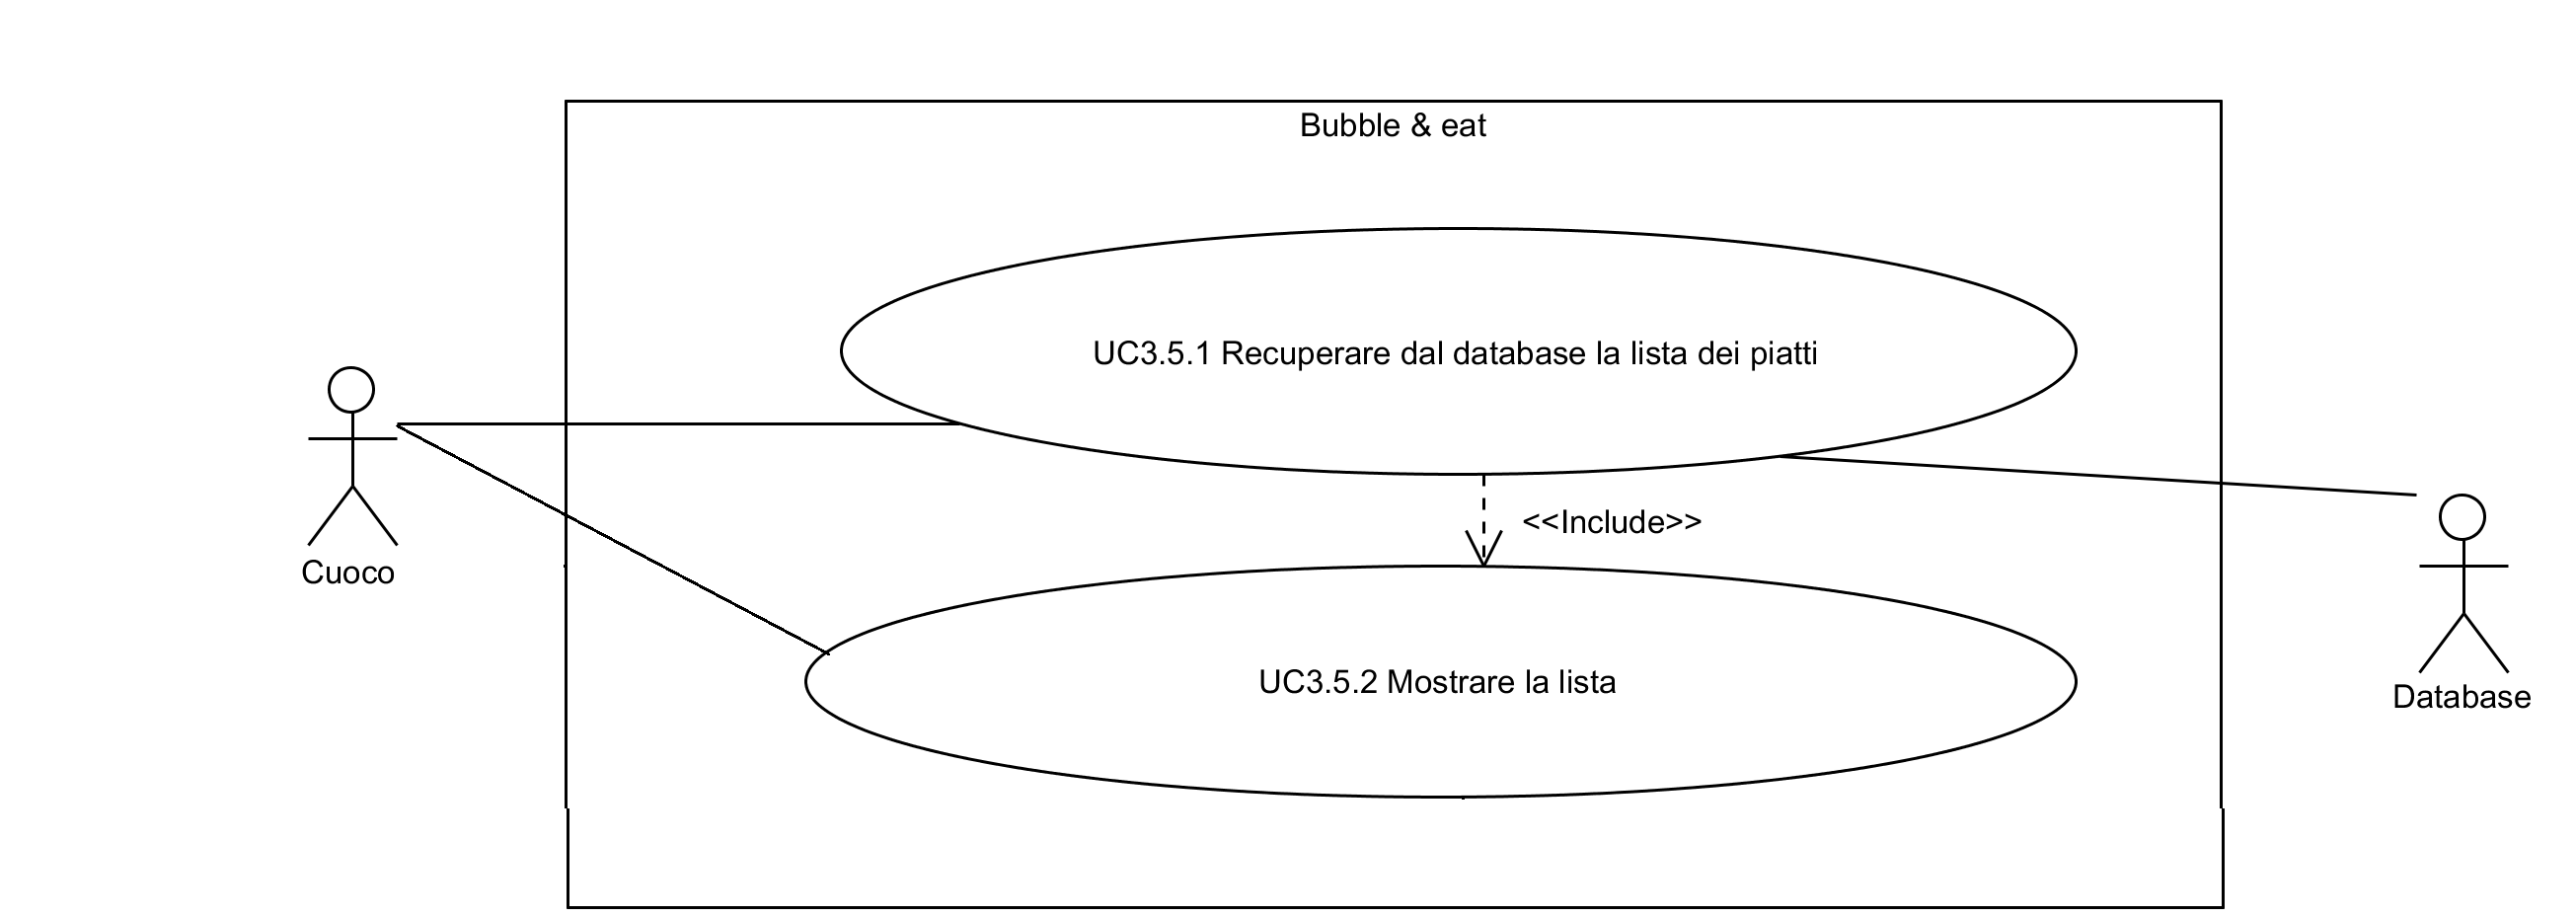
\includegraphics[width=15cm]{../../documenti/AnalisiDeiRequisiti/Diagrammi_img/uc3_5.png}
	\caption{\UCCaption{} Leggere la lista dei piatti da preparare}
\end{figure}

\begin{itemize}
	\item \textbf{Attori:}
	\\Cuoco.
	\item \textbf{Scopo e descrizione:} 
	\\Lo scopo di questa funzionalità è permettere al Cuoco di consultare la lista dei piatti da preparare ottenuta tramite le ordinazioni effettuate dai clienti.
	\item \textbf{Precondizioni:}
	\begin{itemize}
		\item Avere Rocket.Chat.
		\item Avere la bubble del ristorante selezionato.
		\item Avere accesso alla bubble con il ruolo di Cuoco.
	\end{itemize}
	\item \textbf{Flusso principale degli eventi:}
	\begin{itemize}
		\item Il Cuoco seleziona la parte corrispondente della bubble.
		\item Viene recuperata dal database la lista dei piatti \ref{UC3.5.1}.
		\item Viene mostrata la lista all'utente \ref{UC3.5.2}.
	\end{itemize}
	\item \textbf{Post-condizione:}
	\\Il Cuoco è a conoscenza dei piatti ordinati.
\end{itemize}

\UCF{Recuperare dal database la lista dei piatti}{UC3.5.1}

\begin{itemize}
	\item \textbf{Attori:}
	\\Cuoco.
	\item \textbf{Scopo e descrizione:} 
	\\Lo scopo di questa funzionalità è quello di caricare dal database la lista dei piatti da preparare.
	\item \textbf{Precondizioni:}
	\begin{itemize}
		\item Avere Rocket.Chat.
		\item Avere la bubble del ristorante selezionato.
		\item Avere accesso alla bubble con il ruolo di Cuoco.
	\end{itemize}
	\item \textbf{Flusso principale degli eventi:}
	\\Il Cuoco richiede di visualizzare la lista dei piatti da preparare, la bubble carica la lista dal database.
	\item \textbf{Post-condizione:}
	\\La bubble ha recuperato la lista dei piatti da preparare dal database.
\end{itemize}

\UCF{Mostrare la lista}{UC3.5.2}

\begin{itemize}
	\item \textbf{Attori:}
	\\Cuoco.
	\item \textbf{Scopo e descrizione:} 
	\\Lo scopo di questa funzionalità è di far visualizzare al Cuoco la lista dei piatti precedentemente caricata dal database sulla bubble.
	\item \textbf{Precondizioni:}
	\begin{itemize}
		\item Avere Rocket.Chat.
		\item Avere la bubble del ristorante selezionato.
		\item Avere accesso alla bubble con il ruolo di Cuoco.
		\item Aver caricato la lista dei piatti \ref{UC3.5.1}.
	\end{itemize}
	\item \textbf{Flusso principale degli eventi:}
	\\La bubble mostra la lista dei piatti precedentemente memorizzata al Cuoco.
	\item \textbf{Post-condizione:}
	\\Il Cuoco visualizza la lista dei piatti.
\end{itemize}

\UC{Spunta piatti pronti}{UC3.6}

\begin{figure}[H]
	\centering
	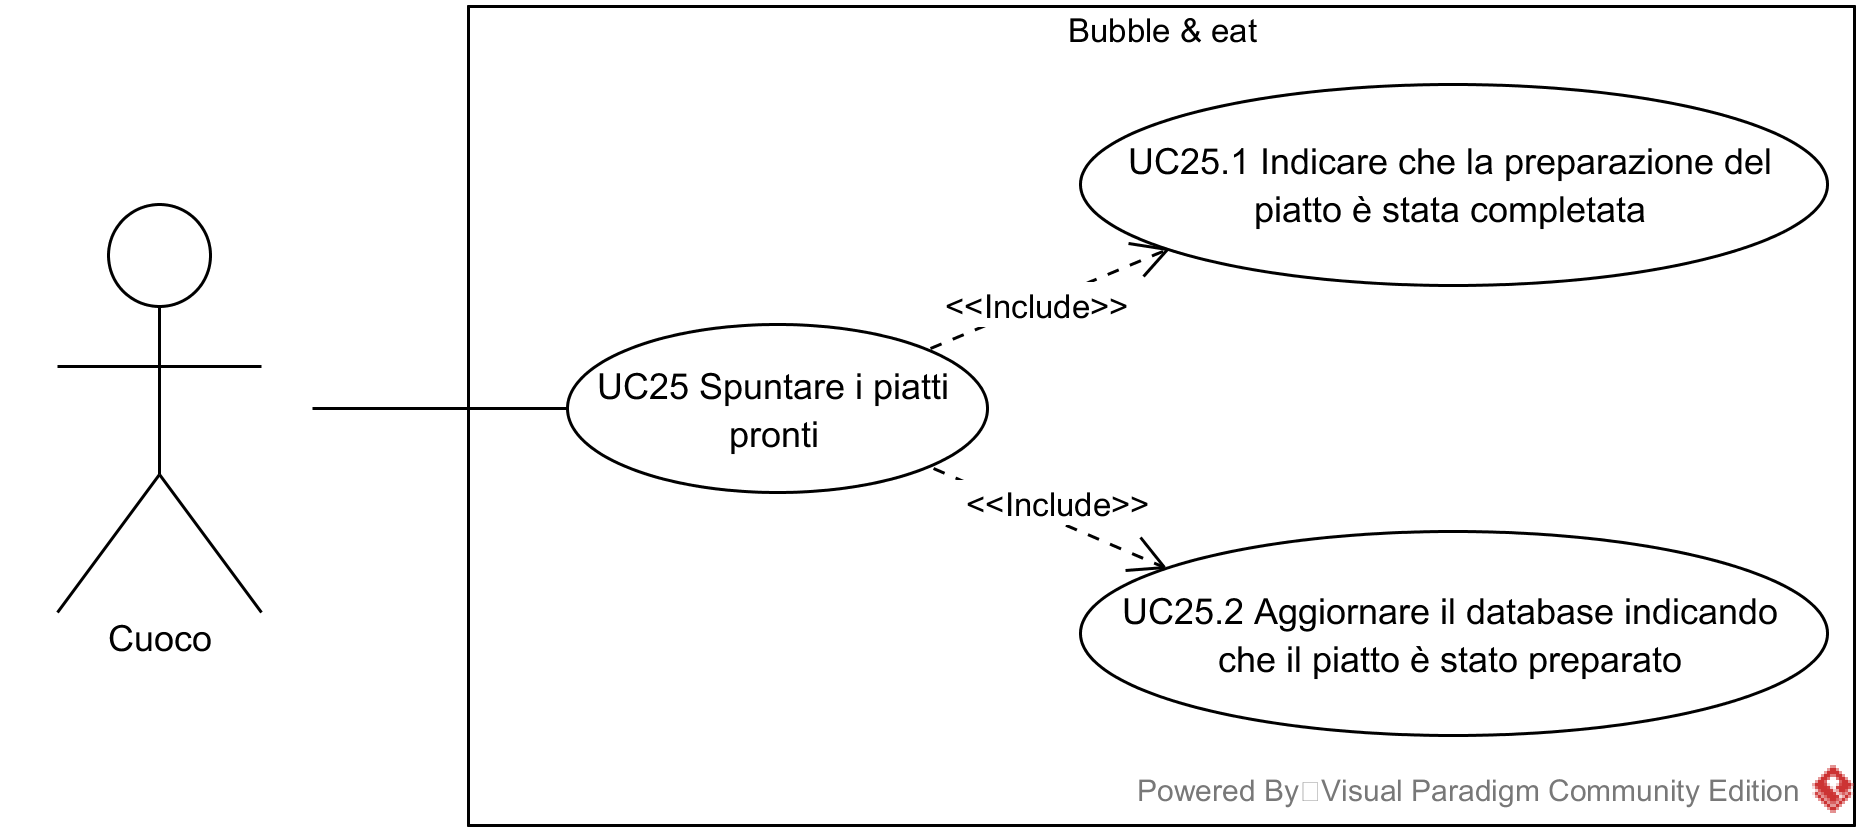
\includegraphics[width=15cm]{../../documenti/AnalisiDeiRequisiti/Diagrammi_img/uc3_6.png}
	\caption{\UCCaption{} Spunta piatti pronti}
\end{figure}

\begin{itemize}
	\item \textbf{Attori:}
	\\Cuoco.
	\item \textbf{Scopo e descrizione:} 
	\\I piatti presenti nella lista possono essere spuntati quando il Cuoco ha finito la loro preparazione.
	\item \textbf{Precondizioni:}
	\begin{itemize}
		\item Avere Rocket.Chat.
		\item Avere la bubble del ristorante selezionato.
		\item Avere accesso alla bubble con il ruolo di Cuoco.
		\item Avere la lista dei piatti da preparare.
	\end{itemize}
	\item \textbf{Flusso principale degli eventi:}
	\begin{itemize}
		\item Il Cuoco indica che ha terminato la preparazione di un piatto \ref{UC3.6.1}.
		\item Il database viene aggiornato con le nuove informazioni \ref{UC3.6.2}.
	\end{itemize}
	\item \textbf{Post-condizione:}
	\\Il piatto è stato spuntato.
\end{itemize}

\UCF{Indicare che la preparazione del piatto è stata completata}{UC3.6.1}

\begin{itemize}
	\item \textbf{Attori:}
	\\Cuoco.
	\item \textbf{Scopo e descrizione:} 
	\\Lo scopo di questa funzionalità è di permettere al Cuoco di indicare che ha completato la preparazione di un piatto.
	\item \textbf{Precondizioni:}
	\begin{itemize}
		\item Avere Rocket.Chat.
		\item Avere la bubble del ristorante selezionato.
		\item Avere accesso alla bubble con il ruolo di Cuoco.
		\item Avere la lista dei piatti da preparare.
		\item Aver precedentemente indicato che si stava preparando un determinato piatto.
	\end{itemize}
	\item \textbf{Flusso principale degli eventi:}
	\\Il Cuoco indica sulla sua lista che ha completato la preparazione del piatto.
	\item \textbf{Post-condizione:}
	\\Il Cuoco ha indicato che ha completato un piatto.
\end{itemize}

\UCF{Aggiornare il database indicando che il piatto è stato preparato}{UC3.6.2}

\begin{itemize}
	\item \textbf{Attori:}
	\\Cuoco.
	\item \textbf{Scopo e descrizione:} 
	\\Lo scopo di questa funzionalità è quello di aggiornare il database in base ai piatti preparati dal Cuoco.
	\item \textbf{Precondizioni:}
	\begin{itemize}
		\item Avere Rocket.Chat.
		\item Avere la bubble del ristorante selezionato.
		\item Avere accesso alla bubble con il ruolo di Cuoco.
		\item Avere preparato dei piatti dalla lista di piatti da preparare.
	\end{itemize}
	\item \textbf{Flusso principale degli eventi:}
	\\I dati sui piatti preparati dal Cuoco vengono aggiornati nel database.
	\item \textbf{Post-condizione:}
	\\I dati nel database sono aggiornati.
\end{itemize}